\chapter{Task 3}
\begin{parlist}
  \item korrigieren() should look at the solution for each question and give it points depending on how correct/incorrect it is.
  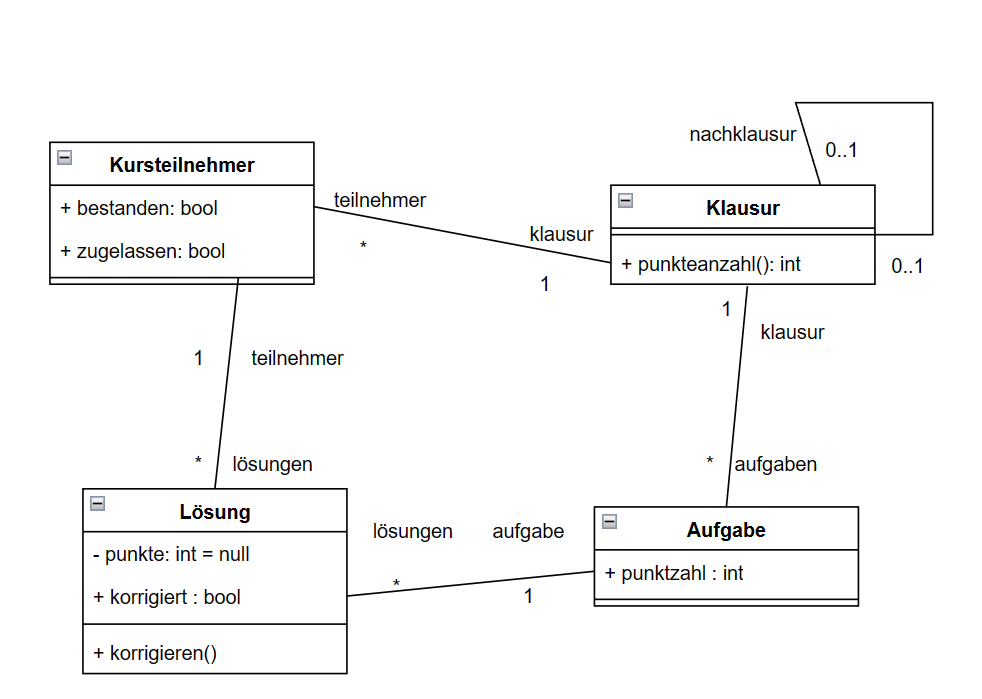
\includegraphics[width=\textwidth]{Immagini/aufg3}
  \item \begin{lstlisting}[language=ocl, frame=trBL]
context Lösung::korrigieren() pre: aufgabe != null
context Lösung::korrigieren() pre: teilnehmer != null
context Lösung::korrigieren() pre: not korrigiert
context Lösung::korrigieren() post: korrigiert = true
context Lösung::korrigieren() post: punkte <= aufgabe.punktzahl
context Lösung::korrigieren() post: punkte >= 0
  \end{lstlisting}
  \item\begin{lstlisting}[language=ocl, frame=trBL]
context Lösung::korrigieren() pre: aufgabe != null
context Lösung::korrigieren() pre: teilnehmer != null
context Lösung::korrigieren() post: korrigiert = true
context Lösung::korrigieren() post: punkte <= aufgabe.punktzahl
context Lösung::korrigieren() post: punkte >= 0
  \end{lstlisting}
  \item\begin{lstlisting}[language=ocl, frame=trBL]
context Klausur::punkteanzahl post: result = aufgaben->collect(punktzahl)->sum()
  \end{lstlisting}
\end{parlist}
